\documentclass[a4paper,12pt]{article}

\input{preamble}

\date{\today}
\author{Никита Лансков}
\title{Стохастические модели и анализ данных\\
Работа по восстановлению зависимости}


\begin{document} % конец преамбулы, начало документа

\maketitle
\tableofcontents

\newpage

\section{Постановка задачи}
Требуется выбрать массив данных с интервальной неопределенностью и восстановить
линейную зависимость.

Модель данных будем искать в классе линейных функций

\begin{equation}
    y = \beta_1 + \beta_2x
\end{equation}

При условии: $\beta_2 > 0$

% Вот тут будет график данных

\section{Параметры модели}

\subsection{Предобработка данных}
\begin{figure}[h!]~\label{fig1}
\centerline{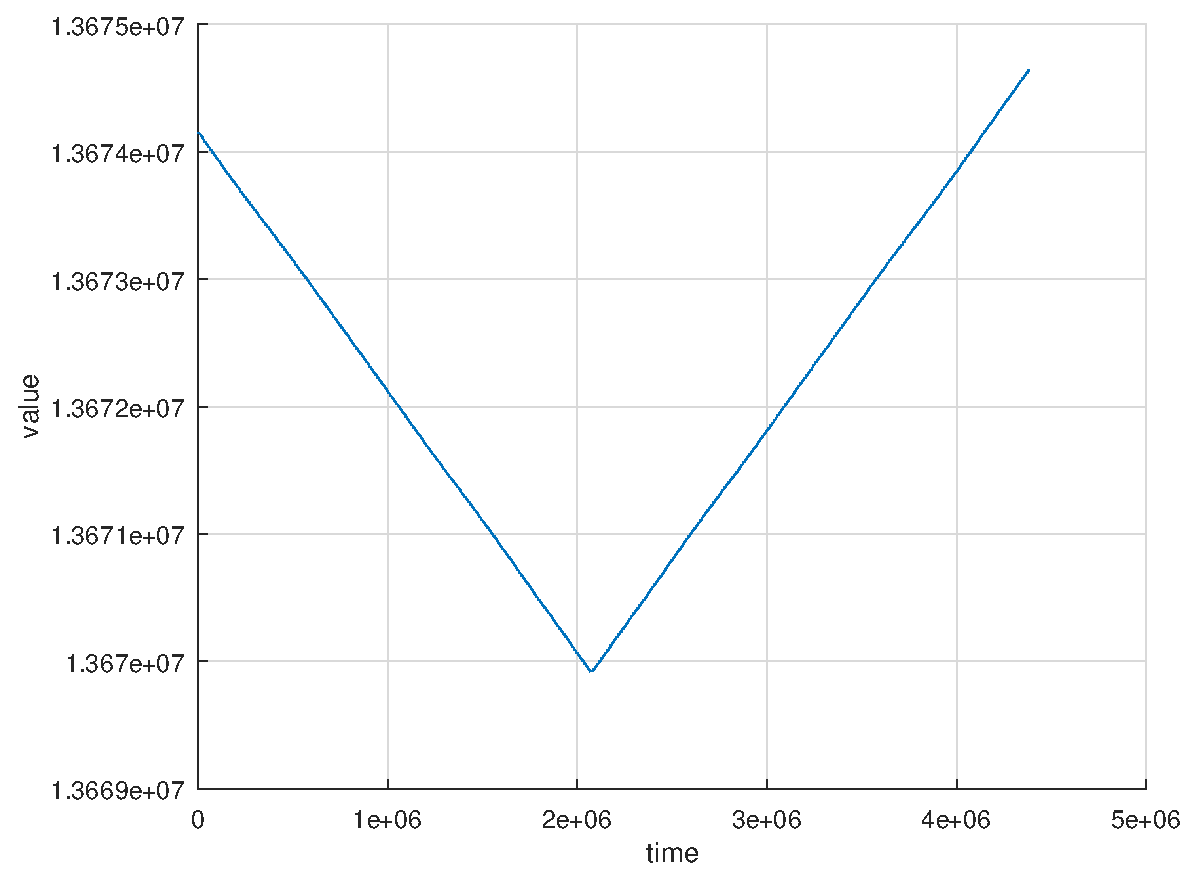
\includegraphics[scale = 0.7]{all_data.eps}}
\caption{Все данные}
\end{figure}
Выберем область, которую будем рассматривать, например: 
$t \in [2.5e^6, 4.3e^6]$

\begin{figure}[h!]~\label{fig2}
\centerline{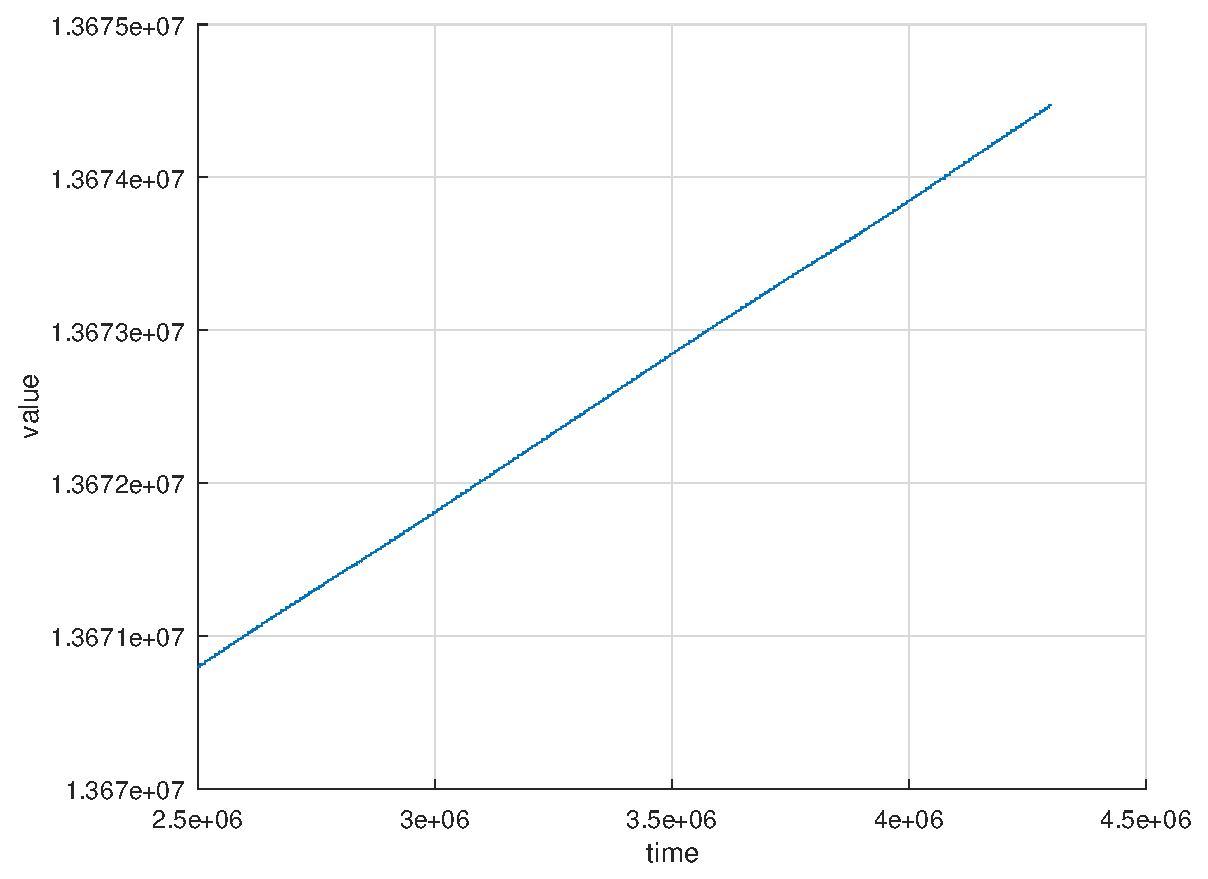
\includegraphics[scale = 0.7]{filtered_data.eps}}
\caption{Выбранный диапазон значени}
\end{figure}
Даллее объединим точки, значения в которых отличаются менее чем на 20.

Ну и в качестве значений нашей небольшой подвыборки возьмем первые 10 точек
на нечетных позициях.

в итоге получим данные следующего вида.

\newpage
\begin{figure}[h!]~\label{fig3}
\centerline{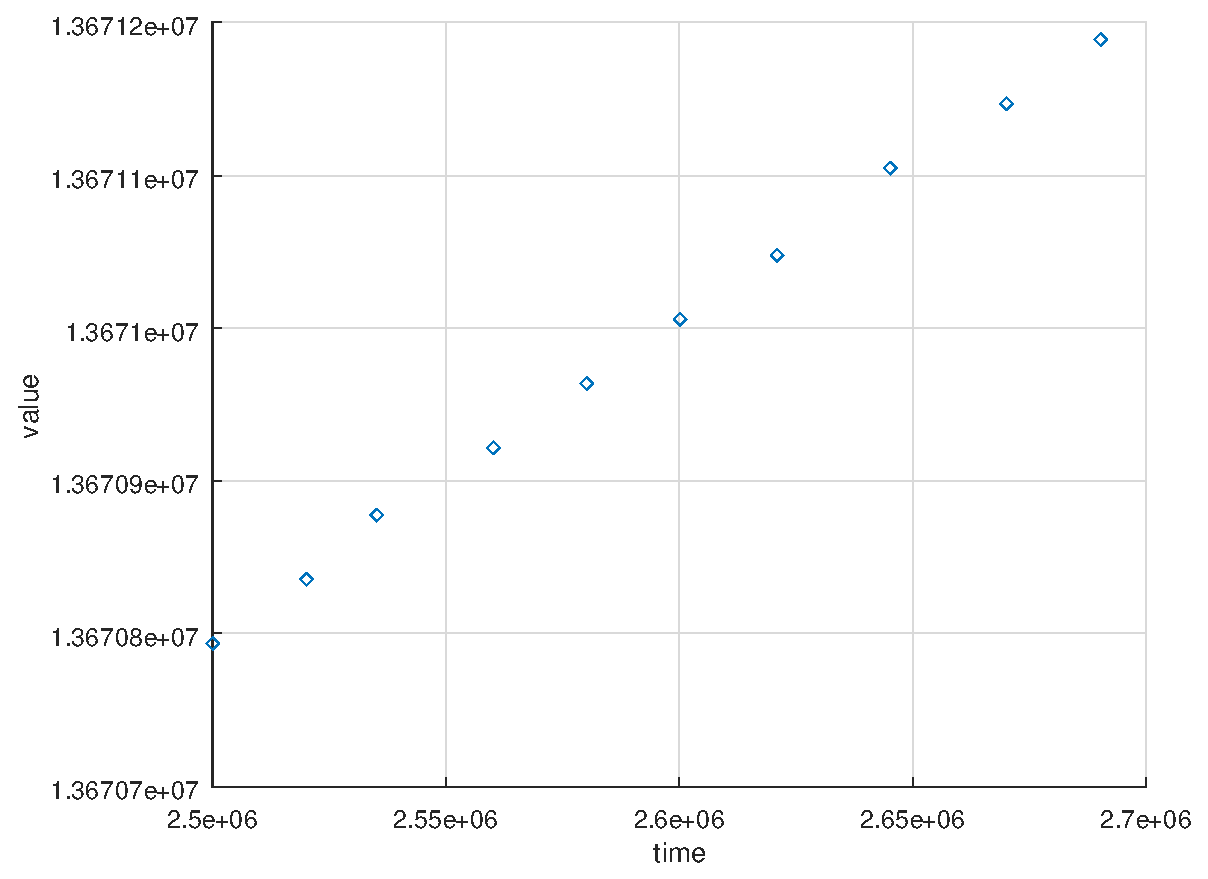
\includegraphics[scale = 0.7]{selected_data.eps}}
\caption{Итоговая выборка из 10 значений}
\end{figure}

\subsection{Линейная модель МНК для точечных значений}

В качестве начальной погрешности возьмем $\varepsilon = 1$, в соответствии с 
последним значащим разрядом в данных.

\begin{figure}[h!]~\label{fig4}
\centerline{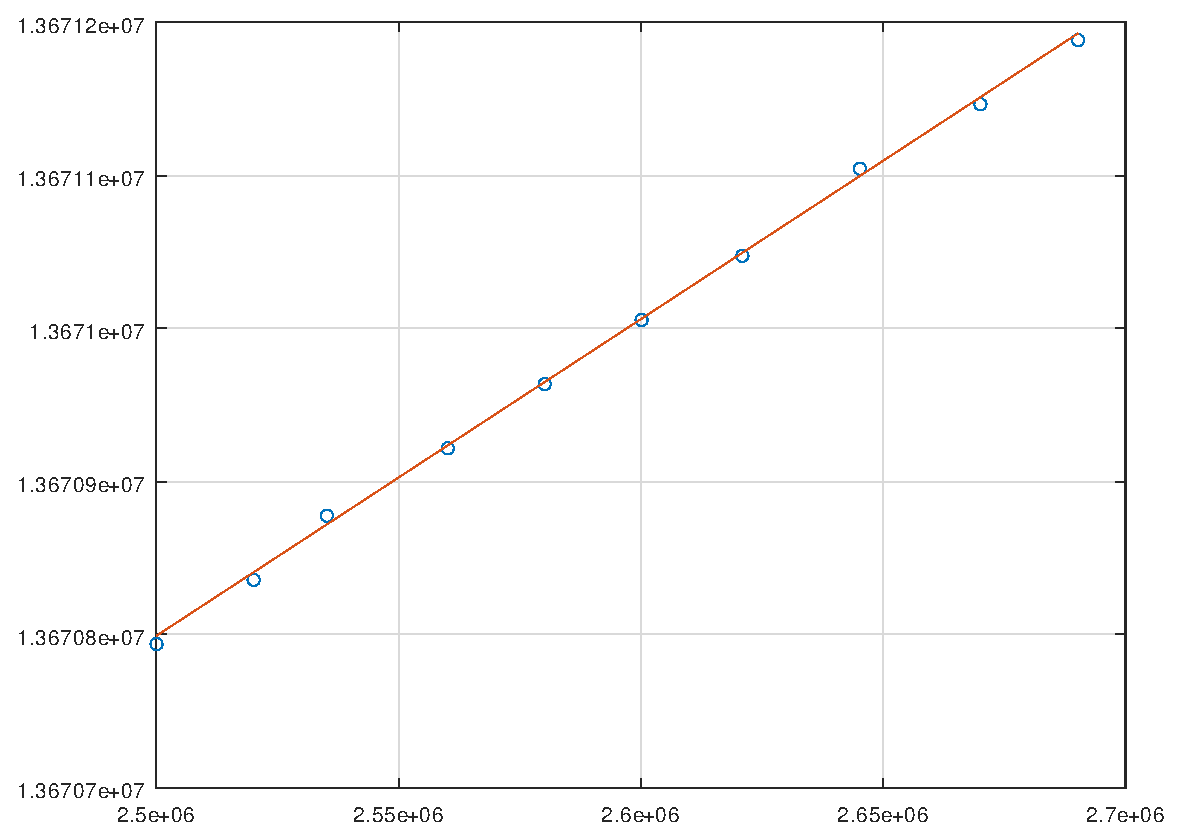
\includegraphics[scale = 0.7]{dot_mnk.eps}}
\caption{МНК}
\end{figure}

Для точечного случая по методу наименьших квадратов получаем следующие
значения параметров:$$ \beta_1=1.3666e^7, \beta_2=2.0722e^{-3} $$

\subsection{Модель для интервального случая}

При переходе к интревальному случаю, обнаруживаем, что информационное множество
оказывается пустым.
Попробуем это исправить, решив задачу оптимизации для уточнения 
погрешности~\cite{baz}.

\begin{equation}
\left\{
\begin{aligned}
    mid~y_i - w_i~\cdot rad~y_i \leq X \beta &\leq mid~y_i + w_i~\cdot rad~y_i, 
    i = \overline{1, m} \\ 
    \sum\limits_{i=1}^m w_i &\rightarrow \min \\
    w_i \geq 0, i &= \overline{1, m}\\
    w, \beta &=~?
\end{aligned}
\end{equation}

Где $X$ - матрица $m \times 2$, в первом столбце единичные значения, а во 
втором значения $x_i$.
$$mid~y_i = y_1,~rad~y_i = \varepsilon_i$$

Полученные значения в задаче оптимизации:
\[
    w = [3.77, 3.12, 7.71, 1.00, 1.00, 1.78, 1.00, 7.87, 1.39, 1.00]
\]
\[
    \beta = [1.3666e^7, 2.0710e^{-3}]
\]

Увеличим погрешность всех измерений:

\[
    rad~y_i = \max\limits_i~w_i \cdot \varepsilon
\]

Построим новое информационное множество параметров модели. Поскольку
информационное множество задачи построения линейной зависимости по интервальным
данным задаётся системой линейных неравенств, то оно представляет собой 
выпуклый многогранник.~\cite{ex} Дополнительно обозначим на графитке центр наибольшей 
диагонали информационного множества и его центр тяжести.


\begin{figure}[h!]~\label{fig5}
\centerline{\includegraphics[scale = 0.7]{info_set_full.eps}}
\caption{Информационное множество}
\end{figure}

\newpage
\section{Коридор совместных зависимостей}

\begin{figure}[h!]~\label{fig6}
\centerline{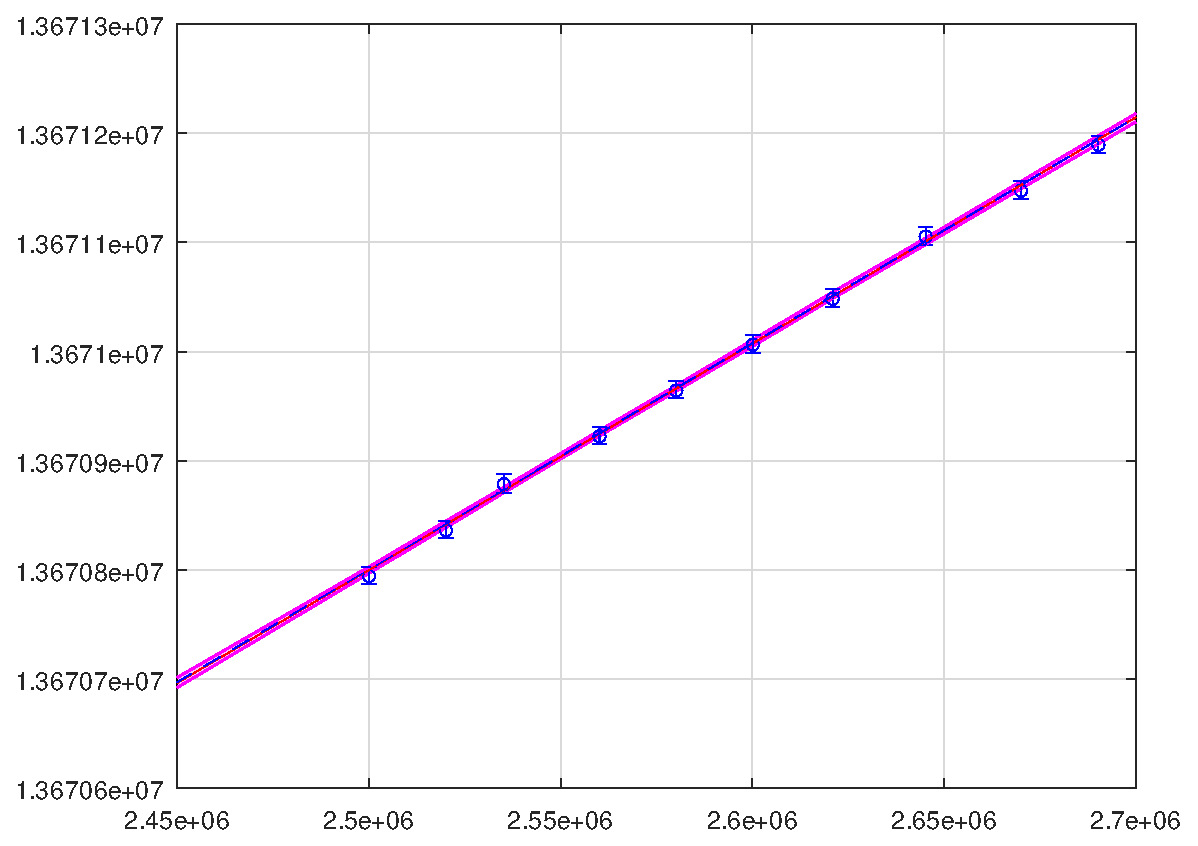
\includegraphics[scale = 0.7]{joint_depth.eps}}
\caption{Коридор совместных зависимостей}
\end{figure}


\newpage
\section{Прогноз за пределы интервала}

При помощи построенной модели:
\[
    \hat{y}(x) = [1.3666e^7, 1.3666e^7] + [2.0342e^{-3}, 2.1079e^{-3}]x   
\]

Спрогнозируем значения для $x_p = [2.75e^6; 2.78e^6; 2.81e^6; 2.86e^6; 2.95e^6]$

\begin{table}[h!]~\label{tb1}
    \begin{center}
        \begin{tabular}{|c|c|c|}
            \hline
                $x_p$ & $y_p$ & $rad~y_p$ \\
            \hline
                $2.75e^6$ & $[1.36713e^7, 1.36713e^7]$ & 6.2748 \\
            \hline
                $2.78e^6$ & $[1.36714e^7, 1.36714e^7]$ & 7.3793 \\
            \hline
                $2.81e^6$ & $[1.36714e^7, 1.36715e^7]$ & 8.4839 \\
            \hline
                $2.86e^6$ & $[1.36715e^7, 1.36716e^7]$ & 10.3249 \\
            \hline
                $2.95e^6$ & $[1.36717e^7, 1.36717e^7]$ & 13.6386 \\
            \hline
        \end{tabular}
    \caption{Прогноз значений}
    \end{center}
\end{table}

\begin{figure}[h!]~\label{fig7}
\centerline{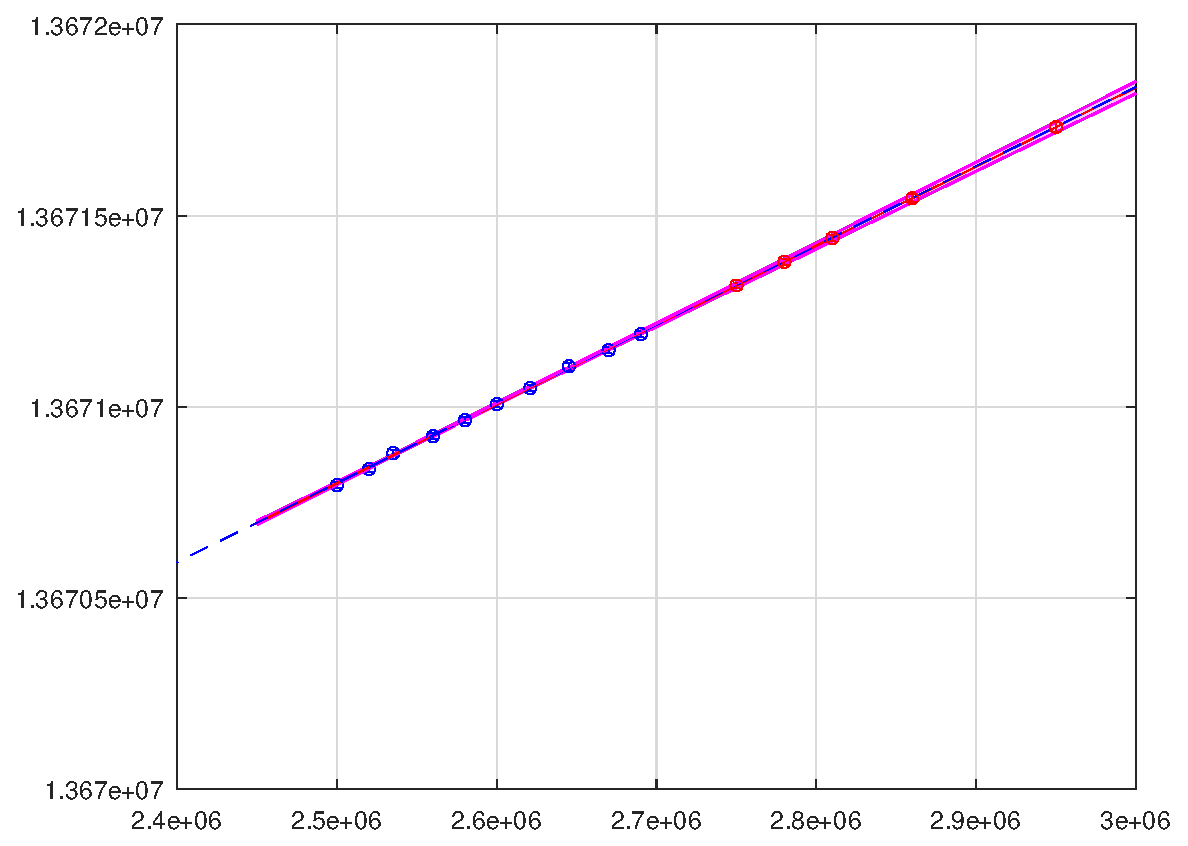
\includegraphics[scale = 0.7]{prediction.eps}}
\caption{Прогноз за пределы интрервала}
\end{figure}

\newpage
\section{Граничные точки множества совместности}

Граничными оказались точки с номерами 1, 3, 8, 9, 10

\begin{figure}[h!]~\label{fig8}
\begin{minipage}[H]{0.45\linewidth}
\center{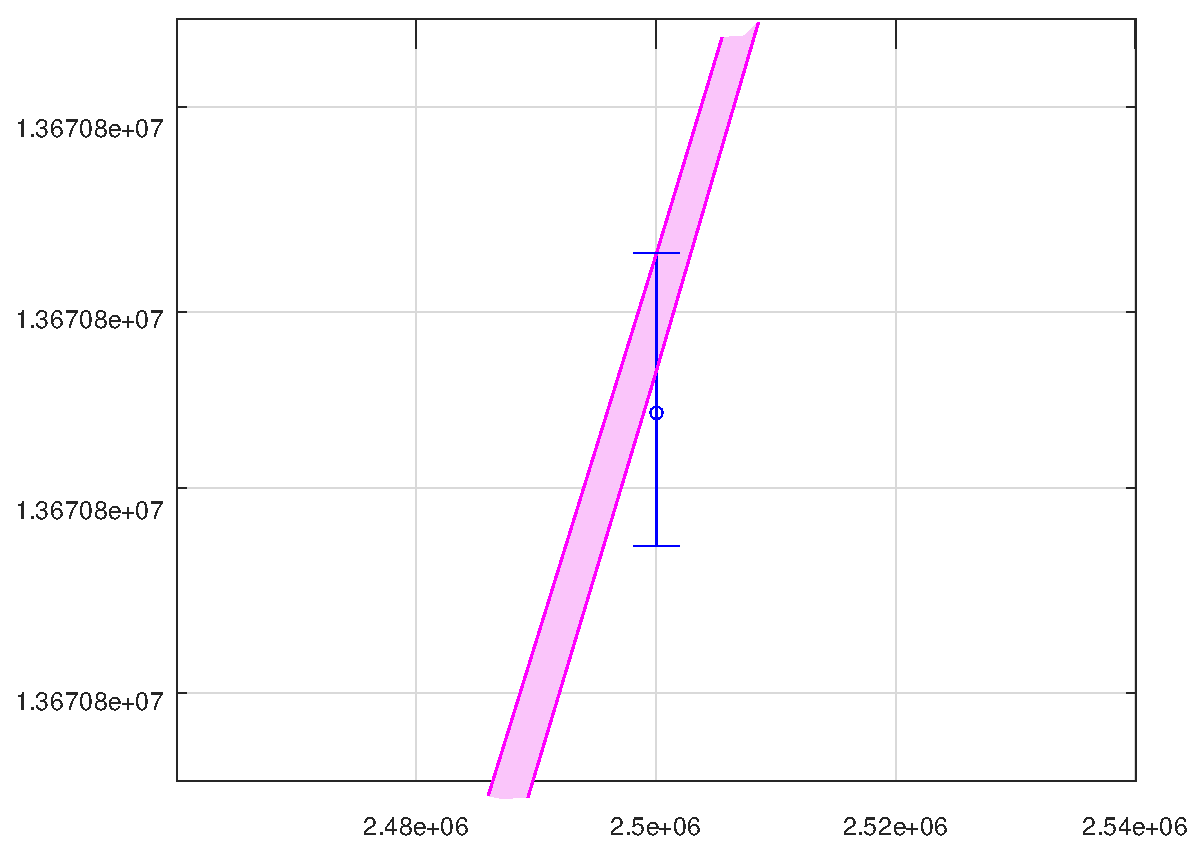
\includegraphics[width=\linewidth]{edge_point_1.eps} \\ 1}
\end{minipage}
\hfill
\begin{minipage}[H]{0.45\linewidth}
\center{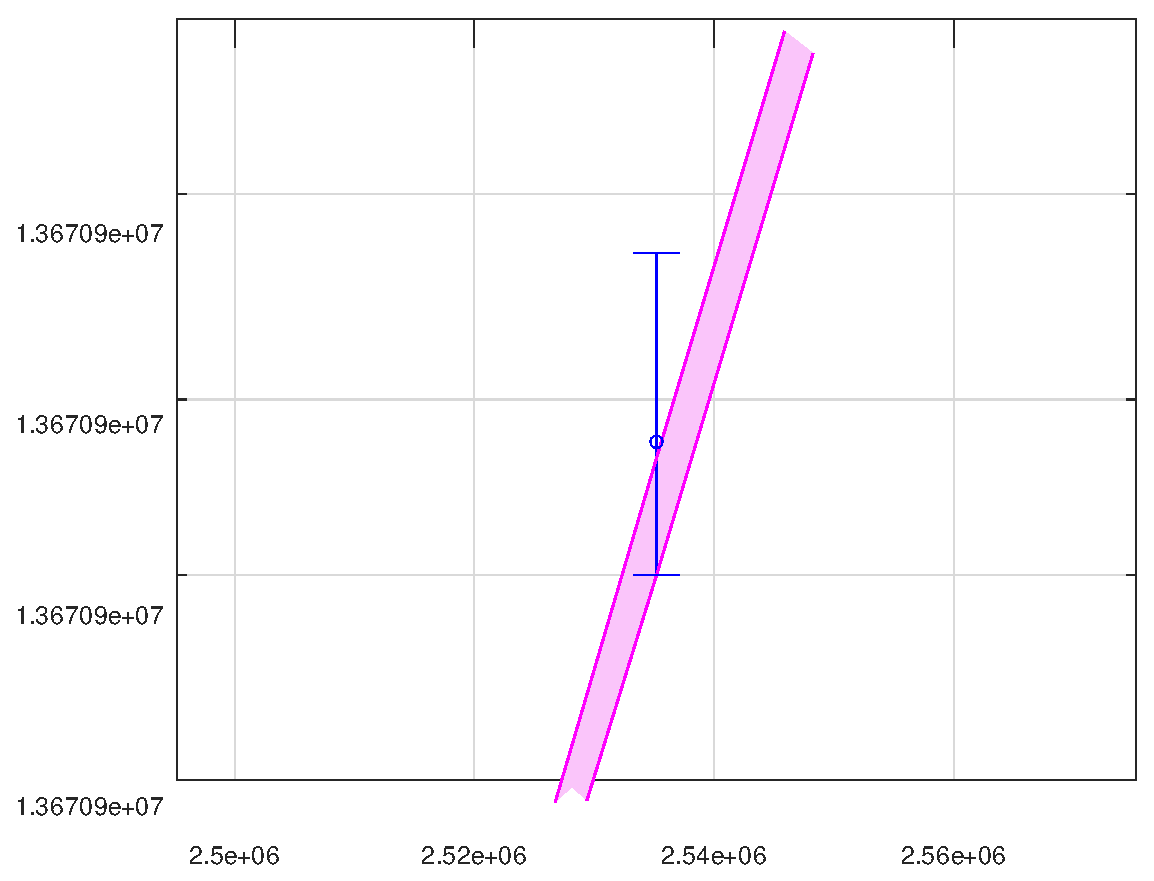
\includegraphics[width=\linewidth]{edge_point_3.eps} \\ 3}
\end{minipage}
\hfill
\begin{minipage}[H]{0.45\linewidth}
\center{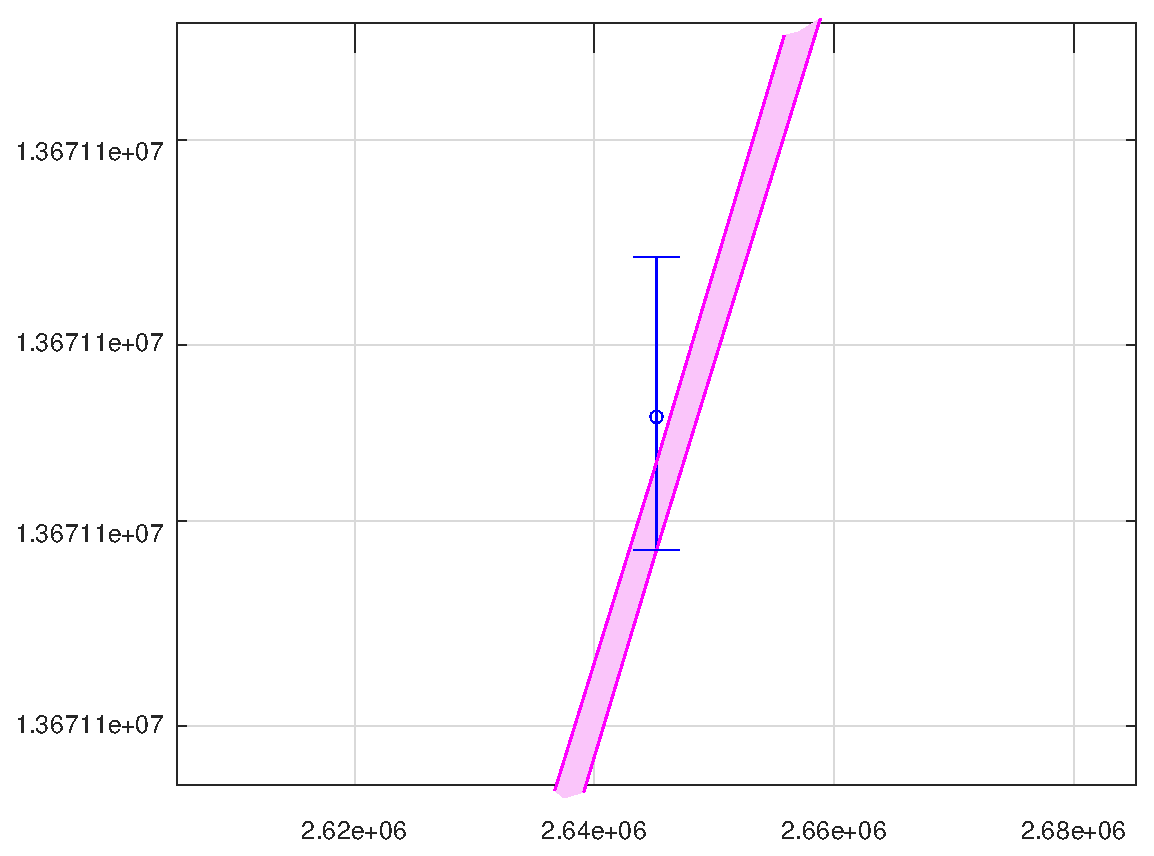
\includegraphics[width=\linewidth]{edge_point_8.eps} \\ 8}
\end{minipage}
\hfill
\begin{minipage}[H]{0.45\linewidth}
\center{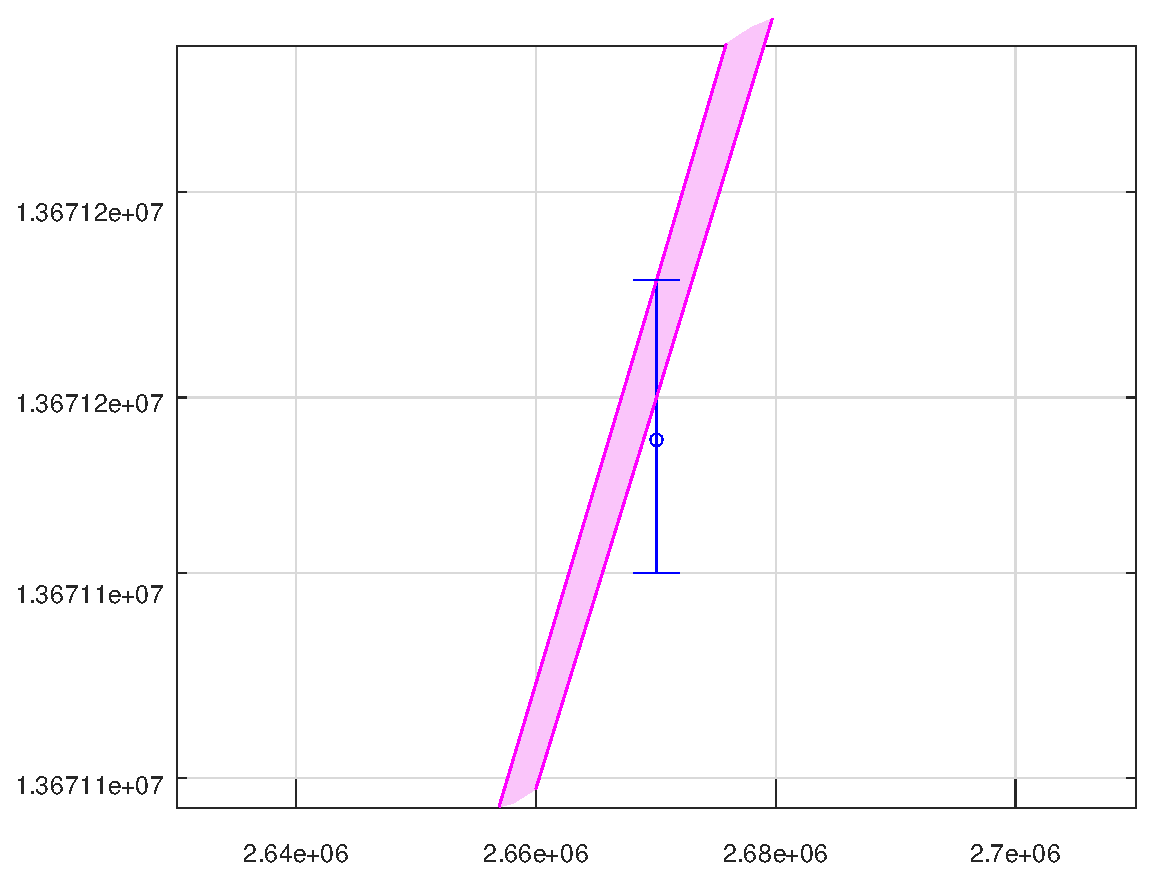
\includegraphics[width=\linewidth]{edge_point_9.eps} \\ 9}
\end{minipage}
\hfill
\begin{minipage}[H]{0.45\linewidth}
\center{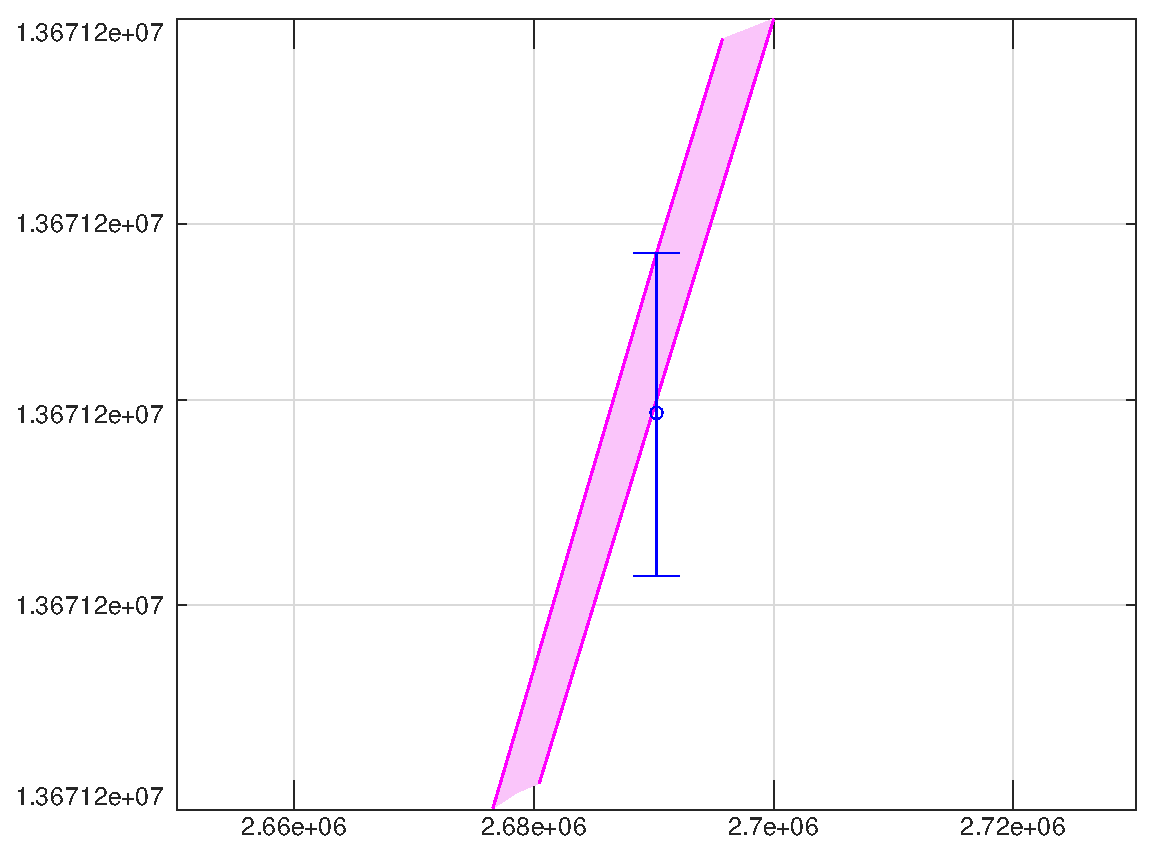
\includegraphics[width=\linewidth]{edge_point_10.eps} \\ 10}
\end{minipage}
\caption{Граничные точки}
\end{figure} 

\pagebreak

Остальные точки не являются граничными:

\begin{figure}[h!]~\label{fig9}
\begin{minipage}[H]{0.45\linewidth}
\center{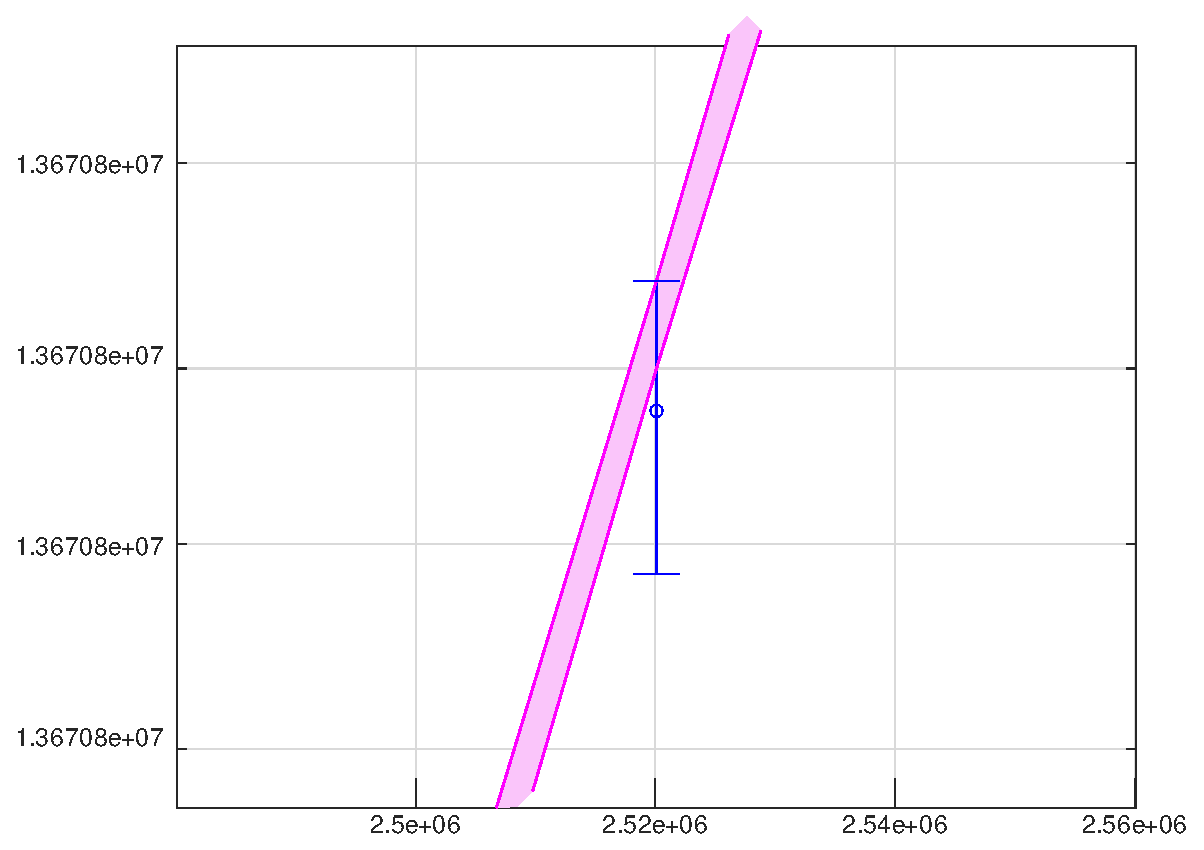
\includegraphics[width=\linewidth]{edge_point_2.eps} \\ 2}
\end{minipage}
\hfill
\begin{minipage}[H]{0.45\linewidth}
\center{\includegraphics[width=\linewidth]{edge_point_4.eps} \\ 4}
\end{minipage}
\hfill
\begin{minipage}[H]{0.45\linewidth}
\center{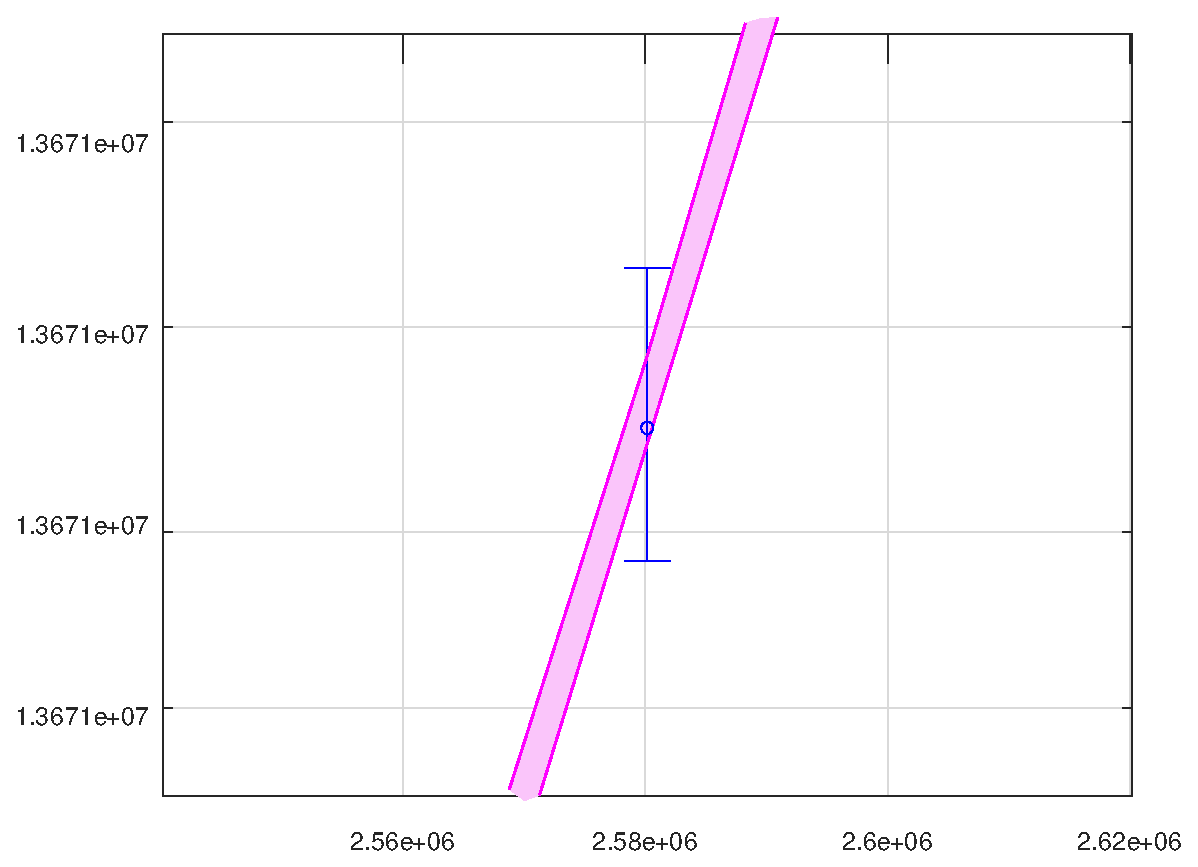
\includegraphics[width=\linewidth]{edge_point_5.eps} \\ 5}
\end{minipage}
\hfill
\begin{minipage}[H]{0.45\linewidth}
\center{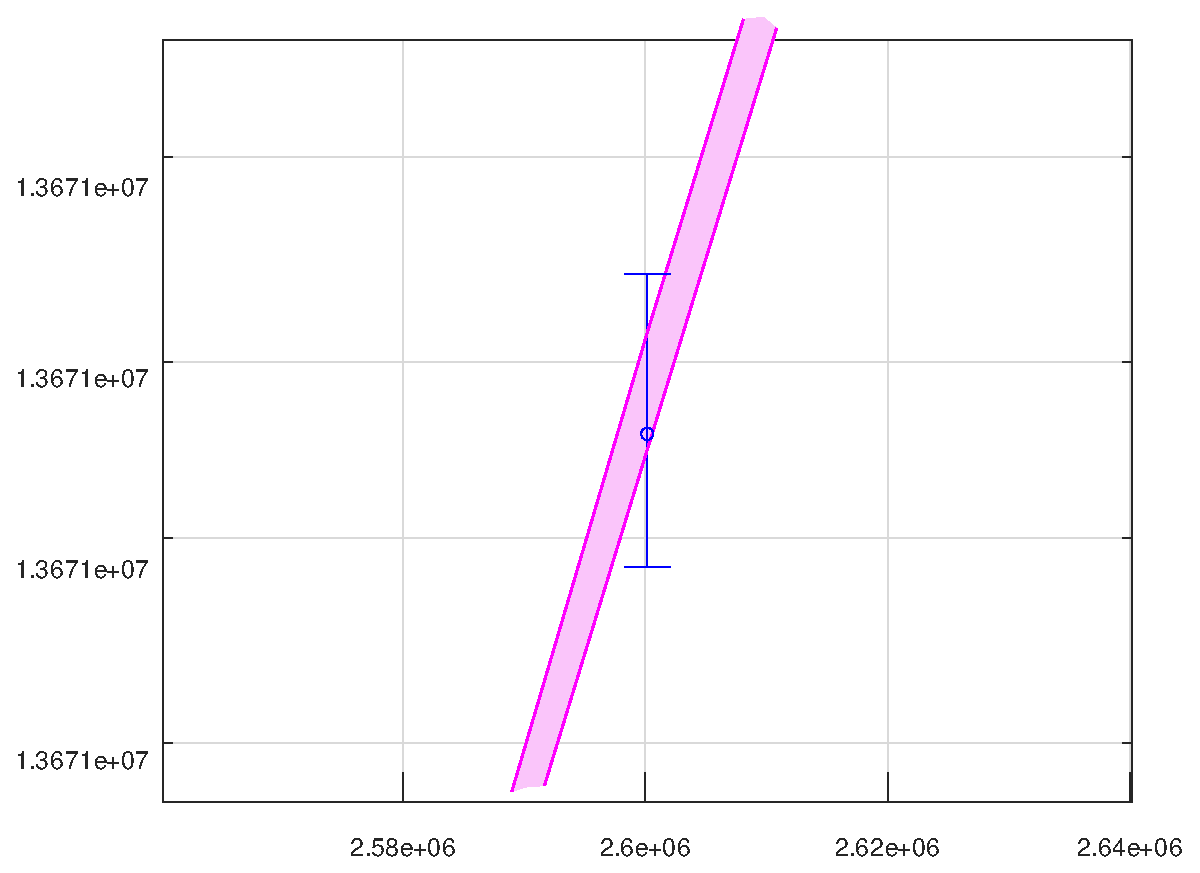
\includegraphics[width=\linewidth]{edge_point_6.eps} \\ 6}
\end{minipage}
\hfill
\begin{minipage}[H]{0.45\linewidth}
\center{\includegraphics[width=\linewidth]{edge_point_7.eps} \\ 7}
\end{minipage}
\caption{Не граничные точки}
\end{figure}

Точка под номером два подозрительно похожа на граничную, но на практике у 
нее слишком большое отклонение от границы, поэтому она была отфильтрована из
граничных.

\newpage
\section{Заключение}

В ходе работы была построена линейная модель данных. Наблюдения
рассматривались сначала как просто точечные, далее – как значения с 
интервальной неопределённостью.

Была задана погрешность наблюдений, однако выборка оказалась несовместной.
Было принято решение, что в выборке отсутствуют выбросы и причина
несовместности – недооценённая погрешность.

Для улучшения оценки погрешности была сформирована и решена задача линейного
программирования. После корректировки выборка стала совместной.

Было получено информационное множество для параметров линейной модели,
построен коридор совместности и обнаружены граничные точки коридора
совместности.
По полученной модели были вычислены прогнозы за пределами области измерений.

Все материалы по данной работе доступны по ссылке:~\cite{github}

\newpage

\listoffigures
\listoftables
\bibliographystyle{unsrt}
\bibliography{references}

\end{document} % конец документа
